\documentclass[a4paper, 14pt]{article}

\usepackage[margin=3cm]{geometry}
\usepackage[utf8]{inputenc}
\usepackage[ngerman]{babel}
\usepackage[autostyle=true,german=quotes]{csquotes}
\usepackage{amsmath}
\usepackage{amssymb}
\usepackage{graphicx}
\usepackage{hyperref}
\usepackage{tikz}
\usepackage{multirow}
\usepackage{array}
% TODO: use \SI everywhere
\usepackage[binary-units=true, per-mode=symbol]{siunitx}
\usetikzlibrary{
	calc
}

\author{Paul Brinkmeier}
\title{Cheatsheet für Einführung in Rechnernetze}

\begin{document}
	\maketitle
	\newpage
	\tableofcontents
	\newpage

	% \raggedright

	\section{Grundlegende Grundlagen}

	\paragraph{Rechnernetz}

	Ein Rechnernetz besteht aus Komponenten und Übertragungsmedien, die diese Komponenten miteinander verbinden.
	Übertragungsmedien realisieren die sogenannten Kommunikationslinks (Übertragungsstrecken) zwischen Komponenten.

	Komponenten sind beispielsweise Computer, Smartphones, Kühlschränke, Router.

	Medien sind beispielsweise Koaxialkabel, Kupferkabel, Glasfaser, Funk.

	\paragraph{Endsystem}

	Endsysteme (Hosts) führen verteilte Anwendungen aus.
	Diese benötigen ein Rechnernetz zur Kommunikation zwischen Anwendungsinstanzen.
	Beispiele für verteilte Anwendungen und Endsysteme: WhatsApp auf Smartphone, E-Mail auf Server, etc.

	\paragraph{Zwischensystem}

	Zwischensysteme leiten Daten im Netz weiter und führen i.d.R. keine verteilten Anwendungen aus.
	Beispiele für Zwischensysteme: Router, Switch.

	\paragraph{(Kommunikations-)Protokoll}

	Protokolle definieren Regeln und Formate für die Kommunikation zwischen zwei oder mehreren Computern sowie die beim Senden und Empfangen von Daten bzw. bei Ereignissen auszuführenden Aktionen.

	\paragraph{(Daten-)Pakete}

	Die von Anwendungen zu sendenden Daten können in kleinere Teile gegliedert werden.
	Diese werden als (Daten-)Pakete bezeichnet.
	Pakete sind aufgebaut aus Metadaten und Nutzdaten.
	Metadaten sind nur für die Abwicklung des Protokolls erforderlich; Nutzdaten sind die eigentlichen für die Anwendung wichtigen Daten.
	I.d.R. werden Pakete in Rechnernetzen unabhängig voneinander bearbeitet.

	\paragraph{Datenrate (Übertragungsrate)}

	Die Datenrate bezeichnet die Geschwindigkeit, mit der Daten zwischen zwei Komponenten übertragen wird.
	Sie wird in bit/s gemessen.
	Größenordnungen: K, M, G, T, etc. \emph{nicht} Ki, Mi, Gi, Ti!

	\subsection{Netzkern und Netzrand}

	\paragraph{Netzkern}

	Der Netzkern besteht aus den Netzen untereinander verbunderer Internet Service Provider (ISPs).
	Er beschäftigt sich vor allem mit der Weiterleitung von Paketen.
	Der Netzkern ist sozusagen das \enquote{Betriebssystem} des Internets.

	\paragraph{Netzrand}

	Der Netzrand besteht aus den Netzen von Endandwendern, bspw. Heimnetze, Firmennetze und Datenzentren.
	Er beherbergt die \enquote{Anwendungen} des Internets.

	\subsection{\enquote{Provider} im Internet}

	\paragraph{Internet-Service-Provider (ISP)}

	ISPs binden Konsumenten an das Internet an.
	Dazu gehören oft tausende Kunden und auch Unternehmen.
	Bspw. Unitymedia, Telekom, 1\&1.

	Verschiedene Größenordnungen: Tier-1-ISP, Regionaler ISP, Zugangs-ISP.

	\subparagraph{Warum hierarchisch?}

	Vernetzung aller $n$ Zugangs-ISPs Verbindungen $\in O(n^2)$ $\leadsto$ skaliert nicht.

	\paragraph{Internet-Exchange-Point (IXP)}

	IXPs sorgen für Datenaustausch zwischen größeren ISPs.
	Es gibt weltweit ca. 400 IXPs.

	\paragraph{Content-Provider}

	Content-Provider erzeugen und stellen Inhalte bereit.
	Sie wollen diese so nah wie möglich an den Netzrand ($\leadsto$ zu den Kunden) bringen.
	Bspw. Google, Netflix, Amazon.

	\subsection{Modellierung}

	\paragraph{Modell}

	Ein Modell ist ein vereinfachtes Abbild der Wirklichkeit.
	Man setzt Modelle ein, um die wesentlichen Aspekte eines Systems darzustellen.
	Die innere Struktur des Systems wird abstrahiert; man modelliert die Interaktion mit dem System (Black-Box).

	\subsubsection{Grundmodell der Kommunikation}

	\begin{itemize}
		\item Sender und Empfänger (je einer oder mehrere).
		\item Abstraktes Medium.
	\end{itemize}

	\paragraph{Abstraktes Medium}
	
	Das Medium verbindet Sender und Empfänger über eine räumliche Distanz.
	Es stellt damit einen (Kommunikations-)Dienst zur Verfügung.
	Den Übergang von Sender/Empfänger zum Medium nennt man Schnittstelle.

	Ein abstraktes Medium trifft keinerlei Aussage über seine konkrete (physische) Umsetzung.

	\subsubsection{Dienstesicht}

	\paragraph{Dienstesicht}

	Betrachtung eines Rechnernetzes als Black-Box.
	Das RN erbringt einen Dienst für seine Nutzer.

	Das RN entspricht hier dem abstrakten Medium.

	\paragraph{Dienst}

	Ein Dienst bündelt zusammengehörige Funktionen und stellt diese einem Nutzer (Dienstnehmer) zur Verfügung.
	Einzelen Teile eines Dienstes können unabhängig voneinander in Anspruch genommen werden.

	Ein \emph{Dienstzugangspunkt} (Service Access Point, SAP) stellt die Schnittstelle zu einem Dienst dar.

	\emph{Dienstnehmer} nehmen eine Dienst in Anspruch.

	\emph{Dienstgeber} (Diensterbringer) stellen einen Dienst zur Verfügung.

	\emph{Dienstprimitive} beschreiben die Interaktionen zwischen Dienstnehmer und Dienstgeber.

	Die \emph{Beschreibung eines Dienstes} reflektiert das Verhalten an den Dienstzugangspunkten zum Dienstgeber.

	\begin{figure}
		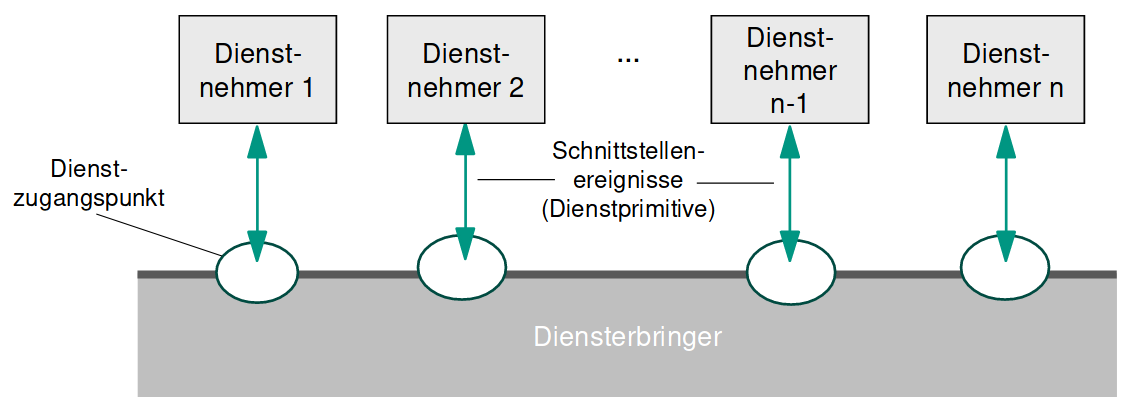
\includegraphics[width=\textwidth]{images/02-services.png}
		\caption{Dienstesicht}
	\end{figure}

	\paragraph{Dienstprimitive}

	\begin{itemize}
		\item \emph{Request} (req) --- Dienstnehmer 1 (DN1) beauftragt Dienstgeber.
		\item \emph{Indication} (ind) --- Dienstgeber benachrichtigt Dienstnehmer 2 (DN2) über Auftrag.
		\item \emph{Response} (res) --- DN2 beantwortet Auftrag.
		\item \emph{Confirmation} (cnd) --- Dienstgeber benachrichtigt DN1 über Abschluss.
	\end{itemize}

	\begin{figure}
		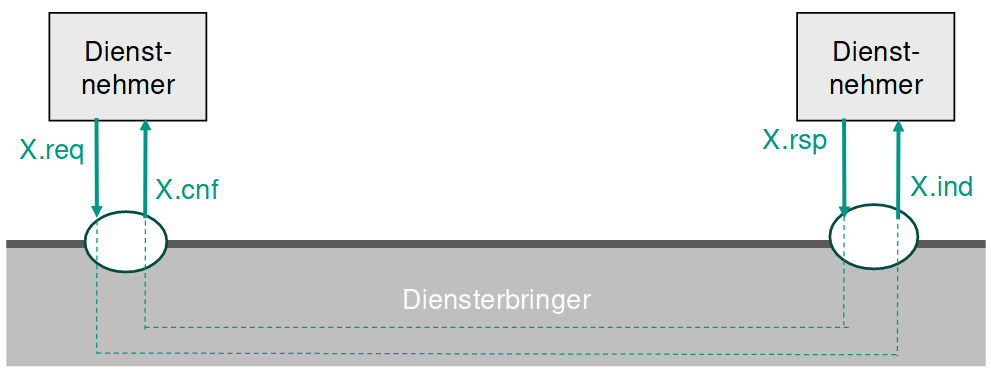
\includegraphics[width=\textwidth]{images/02-primitives.png}
		\caption{Dienstprimitive}
	\end{figure}

	\paragraph{Formen von Diensten}

	\begin{itemize}
		\item Unbestätigter Dienst --- Request (DN1), Indication (DN2).
		\item Bestätigter Dienst --- Request (DN1), Indication (DN2), Response (DN2), Confirmation (DN1).
	\end{itemize}

	\begin{figure}
		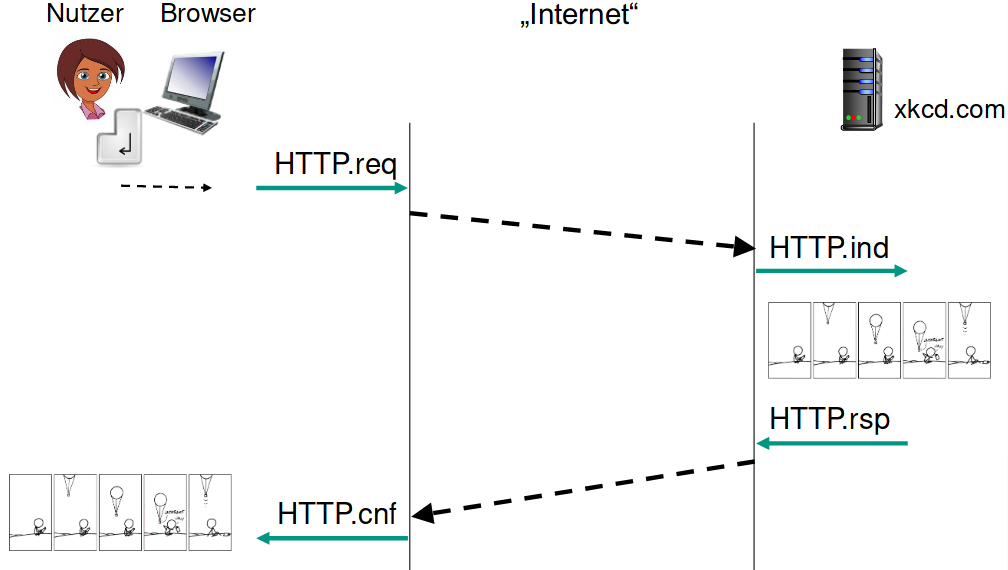
\includegraphics[width=\textwidth]{images/02-http-example.png}
		\caption{Beispiel für einen bestätigten Dienst: HTTP}
	\end{figure}

	\subsection{Zuverlässiger Dienst}

	\paragraph{Zuverlässiger Dienst}

	Bei einem zuverlässigen Dienst gilt am Dienstzugangspunkt des Empfängers folgendes:

	\begin{itemize}
		\item Alle empfangenen Daten sind korrekt.
		\item Alle vom Sender zu empfangenden Daten werden vollständig und in der richtigen Reiehnfolge empfangen.
		\item Es werden keine Duplikate empfangen.
		\item Es werden keine Phantom-Daten empfangen.
	\end{itemize}

	\textbf{Merke}: Zuverlässiger Dienst (ZD) $\neq$ Bestätigter Dienst (BD).
	Es gilt eher BD $\subset$ ZD.
	Bestätigungen sind nur \enquote{ein Baustein} zuverlässiger Dienste.

	\subsection{Schichten}

	\paragraph{Schicht}

	Eine Schicht bündelt zusammengehörige Funktionalitäten, die sich von denen anderer Schichten unterscheiden.
	Schichten sind hierarchisch angeordnet.
	An ihrer Schnittstelle stellt eine Schicht Dienste für die nächst-\enquote{höhere} Schicht bereit und nutzt Dienste der nächst-\enquote{unteren} Schicht.
	Die technische Umsetzung einer Schicht ist an dieser Schnittstelle nicht sichtbar.
	Zur Erbringung ihrere Dienste nutzt eine Schicht die Dienste der darunter liegenden Schicht.

	Protokolle sind innerhalb einer Schicht lokalisiert.

	\begin{figure}
		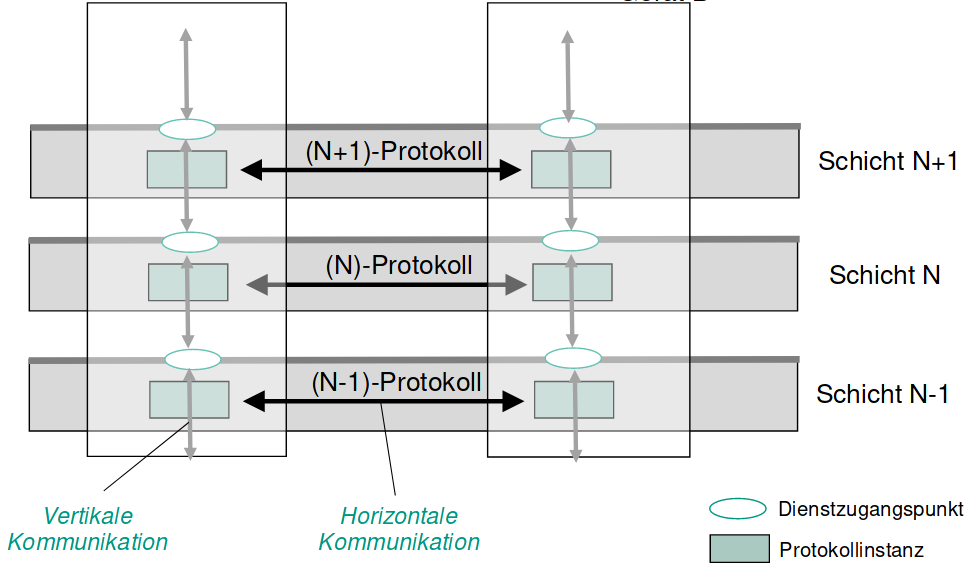
\includegraphics[width=\textwidth]{images/02-layers.png}
		\caption{Protokolle, Dienste, Schichten}
	\end{figure}

	\paragraph{Horizontale Kommunikation}

	Horizontale Kommunikation findet innerhalb einer Schicht zwischen Sender und Empfänger statt.
	Die Protokollinstanzen der Schicht (auf den jeweiligen Geräten) tauschen Daten untereinander aus, um den geforderten Dienst zu erbringen.

	\paragraph{Vertikale Kommunikation}

	Vertikale Kommunikation findet zwischen zwei Schichten innerhalb eines Gerätes statt.
	Protokollinstanz der Schicht $N$ nimmt Dienste der Schicht $N - 1$ in Anspruch oder reichen Daten an Schicht $N + 1$ weiter.

	\subsubsection{Fünf-Schichten-Referenzmodell}

	\begin{figure}
		\begin{center}
			\begin{tikzpicture}[
	>=latex
]
	\node(layers)[inner sep=0]{\Large \begin{tabular}{| c |}
		\hline
		Anwendungsschicht \\
		\hline
		Transportschicht \\
		\hline
		Vermittlungsschicht \\
		\hline
		Sicherungsschicht \\
		\hline
		Physische Schicht \\
		\hline
	\end{tabular}};

	\coordinate (T) at ($(layers.north east) + (1cm, 0)$);
	\coordinate (B) at ($(layers.south east) + (1cm, 0)$);

	\draw[->] (B) -- (T);

	\node[anchor=west] at (T) {Abstraktion hoch};
	\node[anchor=west] at (B) {Abstraktion niedrig};
\end{tikzpicture}

		\end{center}
		\caption{Referenzmodell mit fünf Schichten}
	\end{figure}

	\paragraph{Physische Schicht}

	Zwei direkt über ein Übertragungsmedium beschränkter Länge verbundene Geräte können unstrukturierte Bitfolgen austauschen.
	Eigenschaften dieser Schicht sind:

	\begin{itemize}
		\item Stellt unzuverlässigen Dienst (für die Sicherungsschicht) bereit.
		\item Bits werden nicht gepuffert.
		\item Stark Hardwareabhängig (\enquote{LAN-Kabel}, Glasfaser, WLAN, etc.).
		\item Bei der Übertragung können Störungen auftreten (Paradebeispiel: WLAN).
	\end{itemize}

	\paragraph{Sicherungsschicht}

	Auf dieser Schicht werden zwischen physisch benachbarten Systemen Daten Paketweise (sog. \emph{Rahmen}) übertragen.
	Eigenschaften dieser Schicht sind:

	\begin{itemize}
		\item Ermöglicht Adressierung benachbarter Geräte.
		\item Stellt unzuverlässige und zuverlässige Dienste (Erkennung von Fehlern der physischen Schicht) bereit.
		\item Puffert Daten sowohl beim Sender als auch beim Empfänger.
		\item Abstrahiert physisches Medium.
	\end{itemize}

	\paragraph{Vermittlungsschicht}

	Diese Schicht ermöglicht den Austausch von Daten zwischen (nicht unbedingt) benachbarten Systemen über Zwischensysteme (\emph{Ende-zu-Ende}).
	Pakete nennt man hier typischerweise \emph{Datagramme}.
	Eigenschaften dieser Schicht sind:

	\begin{itemize}
		\item Universale Adressierung von Endsystemen (bspw. IP-Adressen).
		\item Stellt unzuverlässige und zuverlässige Dienste bereit.
		\item Datagramme können in Zwischensystemen gepuffert werden.
		\item Ein Datagramm wird in einem oder mehreren Rahmen der Sicherungsschicht übertragen.
	\end{itemize}

	\paragraph{Transportschicht}

	In dieser Schicht ist die Kommunikation zwischen Anwendungsprozessen auf den Endsystemen gekapselt (\emph{Nutzer-zu-Nutzer}).
	Pakete nennt man hier typischerweise \emph{Datagramme} oder \emph{Segmente}.
	Eigenschaften dieser Schicht sind:

	\begin{itemize}
		\item Adressierung von Anwendungsprozessen auf Endsystemen (\emph{Ports}).
		\item Stellt unzuverlässige (bspw. UDP) und zuverlässige (bspw. TCP) Dienste bereit.
		\item Segmente/Datagramme werden in Endsystemen gepuffert.
		\item Ein Segment/Datagramm wird in einem oder mehreren Datagrammen der Vermittlungsschicht übertragen.
	\end{itemize}

	\paragraph{Anwendungsschicht}

	Über diese Schicht tauschen Anwendungen untereinander \emph{Nachrichten} (bspw. HTTP-Response) aus.
	Je nach Anwendung werden hier zuverlässige oder unzuverlässige Dienste der Transportschicht genutzt.

	\subsubsection{TCP/IP-Referenzmodell}

	Im Internet am weitesten verbreitet (quasi alleinstehend) ist das TCP/IP-Modell.
	Dieses definiert in \href{https://tools.ietf.org/html/rfc1122}{RFC 1122} vier Schichten:

	\begin{center}
		\Large
		\begin{tabular}{| c |}
			\hline
			Anwendungsschicht \\
			\hline
			Transportschicht \\
			\hline
			Internetschicht \\
			\hline
			Netzzugang \\
			\hline
		\end{tabular}
	\end{center}

	Die Internetschicht entspricht der Vermittlungsschicht; Netzzugang kombiniert phyisische und Sicherungsschicht.
	
	\subsubsection{OSI-Referenzmodell}

	Das von der ISO standardisierte OSI-Modell (Open Systems Interconnection Model) definiert sieben Schichten:

	\begin{center}
		\Large
		\begin{tabular}{| c | c}
			\cline{1-1}
			Anwendungsschicht & \multirow{3}{*}{\normalsize Anwendungsorientierte Schichten} \\
			\cline{1-1}
			Darstellungsschicht & \\
			\cline{1-1}
			Sitzungsschicht & \\
			\hline
			Transportschicht & \multirow{4}{*}{\normalsize Transportorientierte Schichten} \\
			\cline{1-1}
			Vermittlungsschicht & \\
			\cline{1-1}
			Sicherungsschicht & \\
			\cline{1-1}
			Physische Schicht & \\
			\cline{1-1}
		\end{tabular}
	\end{center}

	\paragraph{Transportorientierte Schichten}

	Transportorientierte Schichten befassen sich mit der Übertragung von Daten zwischen Anwendungen.
	Die Semantik der übertragenen Daten spielt dabei keine Rolle.

	\paragraph{Anwendungsorientierte Schichten}

	Hier werden Anwendungsbezogene Protokolle abgewickelt.
	Die Semantik der übertragenen Daten ist wichtig.

	\begin{itemize}
		\item \emph{Sitzungsschicht} --- Bietet Nichtunterbrechbarkeit von Kommunikationsbeziehungen.
		\item \emph{Darstellungsschicht} --- Vereinheitlicht Darstellung der Daten über heterogene Systeme hinweg (bspw. Litte- vs. Big-Endian).
		\item \emph{Anwendungsschicht} --- Austausch von anwendungsspezifischen Daten.
	\end{itemize}

	\subsubsection{TCP/IP vs. OSI}

	\begin{itemize}
		\item Netzzugang $\Leftrightarrow$ OSI-Schichten 1 und 2 (physische Schicht, Sicherungsschicht).
		\item Schichten 3 und 4 (Vermittlungsschicht, Transportschicht) sind identisch.
		\item Anwendungsschicht $\Leftrightarrow$ OSI-Schichten 5 bis 7 (Sitzungs-, Darstellungs- und Anwendungsschicht).
	\end{itemize}

	Beim TCP/IP-Referenzmodell wird weniger granular zwischen den Schichten unterschieden.
	Das liegt daran, dass dieses Modell sich eher mit der Zeit aus Prototypen entwickelt hat, als dass es entworfen worden wäre.

	\section{Physische Schicht}

	\subsection{Abstraktes Modell nach Shannon}
	\label{sec:shannon}

	Allgemeine Erkenntnisse, die für alle Arten der Datenübertragung gelten (bspw. Morsen, Telefon, WhatsApp).
	Sender, Empfänger und Kanal sind hier Komponenten der physischen Schicht.

	\paragraph{Informationsquelle}

	Liefert Nachricht in Form einer Bitfolge in vorgegebenem Takt an den Sender.

	\paragraph{Sender}

	Wandelt Nachricht in Signal um und sendet dieses auf den Kanal.

	\paragraph{Kanal}

	Das Medium wird hier als (Übertragungs-)Kanal bezeichnet.
	Eine \emph{Störquelle} kann das Signal beeinflussen.

	\paragraph{Empfänger}

	Rekonstruiert Nachricht aus dem Empfangssignal und übergibt sie der \emph{Informationssenke}.

	\begin{figure}
		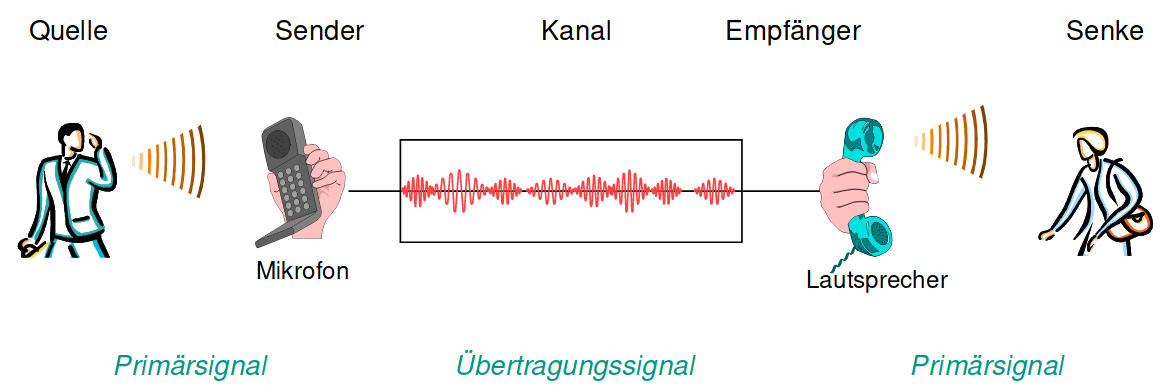
\includegraphics[width=\textwidth]{images/03-shannon-telephone.png}
		\caption{Abstraktes Modell nach Shannon am Beispiel der Telefonie}
	\end{figure}

	\subsection{Medium}

	Das Medium (der Kanal) verbindet auf der physischen Schicht physisch benachbarte Geräte.
	Die Distanz zwischen den Geräten muss überbrückbar sein.
	Um die überbrückbare Distanz zu erhöhen, kommen sogenannte Repeater zum Einsatz, die das Signal verstärken.
	Netze können verschiedenste Medien verwenden; beispielsweise WLAN, UMTS, Kupferkabel oder Glasfaser.

	\subsection{Signal}

	Mit einem Signal können Informationen übertragen werden.
	Formal ist ein Signal eine Funktion $s : T \to V$.
	Zum Zeitpunkt $t$ nimmt das Signal den (Signal-)Wert $s(t)$ ein.

	Signale werden als zeit- und wert-kontinuierlich oder -diskret klassifiziert.
	Diskret heißt hierbei salopp gesagt $T\text{ bzw. }V = \mathbb{Z}$; kontinuierlich heißt $T\text{ bzw. }V = \mathbb{R}$.

	\begin{figure}
		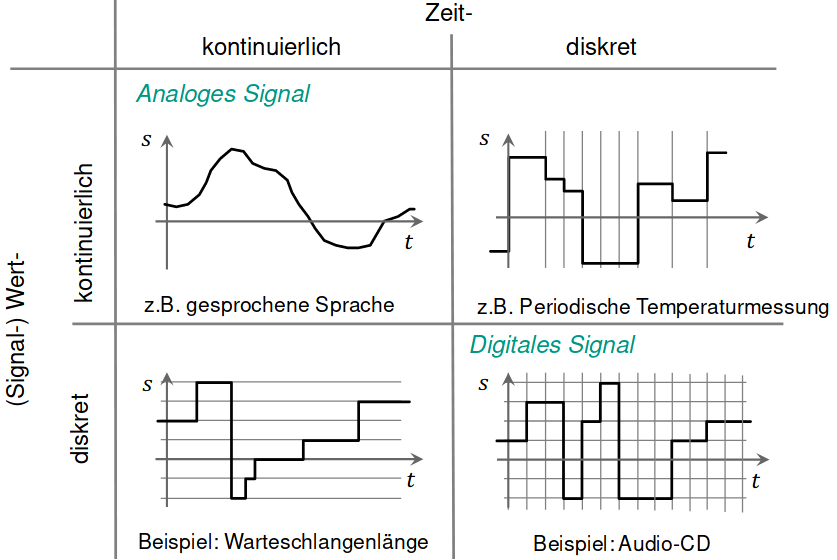
\includegraphics[width=\textwidth]{images/03-signal-classification.png}
		\caption{Klassifizierung von Signalen}
	\end{figure}

	\subsubsection{Digitales Signal}

	Ein digitales Signal ist sowohl zeit- als auch wert-diskret.

	\paragraph{Isochrones digitales Signal}

	Bei einem isochronen digitalen Signal erfolgen Wechsel des Signalwertes nur zum Schritttakt.

	\subsubsection{Analoges Signal}

	Ein analoges Signal ist sowohl zeit- als auch wert-kontinuierlich.

	\paragraph{Periodische Signale}

	Periodische Signale haben eine \emph{Periodendauer} $T$, d.h. der Signalwert wiederholte sich alle $T$ Zeiteinheiten:

	\begin{equation*}
		\forall n \in \mathbb{N} : s(t) = s(t + n \times T)
	\end{equation*}

	Die \emph{Frequenz} $f$ eines periodischen Signals ist definiert als $f = \frac{1}{T}$.

	Merke (aus HM): eine periodische Funktion lässt sich als Summe von Sinus- und Kosinusfunktionen schrieben (Fourier-Reihe).

	Wichtige Parameter der Sinus- und Kosinusfunktionen sind deren Amplitude, Frequenz und Phase.

	\begin{figure}
		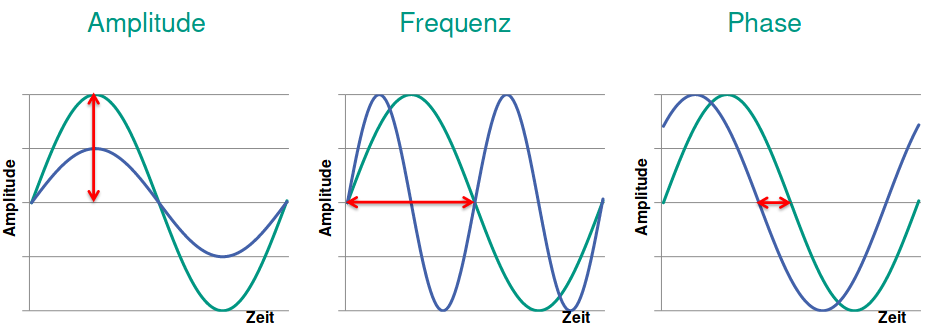
\includegraphics[width=\textwidth]{images/03-trig.png}
		\caption{Parameter trigonometrischer Funktionen}
	\end{figure}

	\subsection{Shannonsche Kanalkapazität}

	\begin{align*}
		C &= B \times \log_2\left(1 + \frac{S}{N}\right)\text{bit} \\
		\frac{S}{N} &= 10 \times \log_{10}\frac{\text{\tiny Signalenergie}}{\text{\tiny Störenergie}}
	\end{align*}

	\begin{itemize}
		\item $C$: Kanalkapazität in bit/s.
		\item $B$: Bandbreite in Hz.
		\item $\frac{S}{N}$: Verhältnis Signal- zu Störenergie.
	\end{itemize}

	Die Kanalkapazität beschreibt die maximale Datenrate, die aufgrund der gegebenen Randbedingungen über einen längeren Zeitraum hinweg aufrecht erhalten werden kann.

	\paragraph{Beispiel:}

	Gegeben sei die Bandbreite $B = 4\text{kHz}$ und das Verhältnis der Signal- zur Störenergie $30\text{dB} \Rightarrow \frac{S}{N} = 10^3$. Also:

	\begin{equation*}
		C = 4\text{kHz} \times \log_2\left(1 + 10^3\right)\text{bit} \approx 40\text{kbit/s}
	\end{equation*}

	\subsection{Modulation und Leitungscodierung}

	Der Sender erhält von der Informationsquelle die Nachricht in Form einer Bitfolge und erzeugt daraus ein phyisisches Signal.
	Innerhalb des Senders agieren der Leitungscodierer und der Modulator.

	\paragraph{Leitungscodierer}

	Der Leitungscodierer bereitet der Bitstrom für die Übertragung vor (bspw. fehlerkorrigierende Codes).

	\paragraph{Modulator}

	Der Modulator bildet aus der codierten Nachricht die physischen Signale.

	\subsection{Modulation}

	Durch Modulation (Veränderung) sinusförmiger Trägersignale wird ein zu übertragendes Nutzsignal für die physische Übertragung ausbereitet.
	Ein zu sendendes digitales Signal wird zur Übertragung in ein analoges überführt.

	\subsubsection{Amplitudenumtastung}

	Hierbei wird die Amplitude des Trägersignals verändert.
	In ihrer einfachsten Form besteht Amplitudenumtastung aus dem Ein- und Ausschalten (zur Übertragung einer 1 bzw. einer 0) des Trägersignals.

	Amplitudenumtastung ist leicht zu implementieren, benötigt wenig Bandbreite, ist aber anfällig für Störungen.

	\subsubsection{Frequenzumtastung}

	Hierbei wird jedem möglichen Signalwert (bspw. 0 und 1) eine Frequenz zugewiesen.

	Frequenzumtastung benötigt eine größere Bandbreite als Amplitudenumtastung.

	\subsubsection{Phasenumtastung}

	Bei Phasenumtastung wird jedem möglichen Signalwert eine bestimmten Phase der Sinusfunktion zugeordnet.

	Phasenumtastung ist zwar komplex in der Umsetzung, jedoch relativ störungssicher.

	\subsection{Leitungscodierung}

	\subsubsection{Codierung}

	Seien $A$ und $B$ endliche Alphabete.
	Eine Codierung ist eine injektive Abbildung $c : A^+ \to B^+$.
	Man nennt $A$ das \emph{Quellenalphabet} und $B$ das \emph{Codealphabet} von $c$.

	\paragraph{Beispiel Morsecode}

	\begin{align*}
		A &= \{\text{A}, ..., \text{Z}, 0, ..., 9, \text{\emph{Punkt}}, \text{\emph{Komma}}, \text{?}\} \\
		B &= \{\bullet-, ..., --\bullet\bullet, ...\} \\
		\\
		c(\text{A}) &= \bullet- \\
		c(\text{Z}) &= --\bullet\bullet \\
		c(\text{SAAAS}) &= \bullet\bullet\bullet\bullet-\bullet-\bullet-\bullet\bullet\bullet
	\end{align*}

	\paragraph{Code}

	Sei $c$ eine Codierung.
	Der von $c$ erzeugte Code ist die Menge

	\begin{equation*}
		C := c(A) = \{ c(z) : z \in A \}
	\end{equation*}

	$c(z) \in B$ nennt man das Codewort eines Zeichens $w \in A$.

	\subsubsection{Mehrwertige Digitalsignale}

	Ein binäres Digitalsignal ist zeit- und wert-diskret.
	Es kann nur zwei Werte annehmen: 0 und 1.
	Ein mehrwertiges Digitalsignal ist zeit- und wert-diskret und kann mehr als zwei Werte annehmen.
	Beispielsweise kann ein quaternäres Signal 4 verschiedene Signalwerte annehmen und damit $\log_2{}4 = 2$ Bit pro Schrittdauer darstellen.

	\subsubsection{Baudrate}

	\paragraph{Übertragungsgeschwindigkeit}
	
	Die Übertragungsgeschwindigkeit (Datenrate) bezeichnet die Anzahl der übertragenen Bits in einer Schrittdauer in bit/s.

	\paragraph{Schrittgeschwindigkeit}

	Die Schrittgeschwindigkeit (Baudrate) bezeichnet die Anzahl der Signalwertwechsel innerhalb eines Schrittes in baud ($=$ bit/s).

	\begin{figure}
		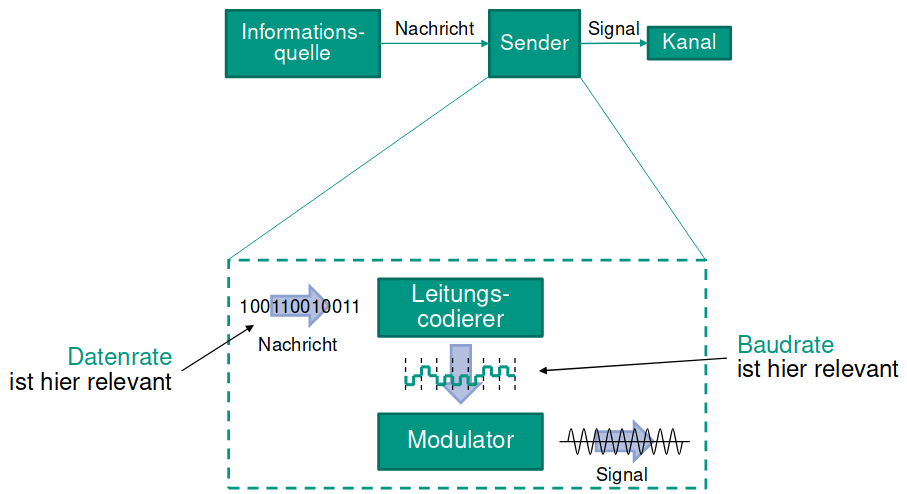
\includegraphics[width=\textwidth]{images/03-baudrate-datarate.png}
		\caption{Baudrate und Datenrate}
	\end{figure}

	\subsection{Leitungscodes}

	Ziele von Leitungscodes sind:

	\paragraph{Taktrückgewinnung}

	Sender um Empfänger verfügen i.d.R. über keinen gemeinsamen Takt.
	Der Empfänger sollte aus den Signalwerten den Takt rekonstruieren können.
	Dies sollte unabhängig vom Inhalt der übertragenen Daten möglich sein.

	\paragraph{Niedrige Baudrate}

	Anzahl der Signalwertwechsel pro Schrittdauer gering halten.

	\paragraph{Geringe Komplexität}

	Kosten, Baugröße, Energieaufnahme, etc. sollten gering sein.

	% TODO: Gleichstromzeug

	\subsubsection{NRZ}

	Bei NRZ (Non-Return to Zero) werden die Symbolwerte durch die Signalwerte bestimmt.
	Eine 1 (0) in der Nachricht wird als hoher (niedriger) Pegel über ein gesamtes Taktintervall codiert.
	Signalwertwechsel erfolgen an den Taktgrenzen; die Erkennung des Signals erfolgt direkt durch auslesen des Pegels.

	\begin{figure}
		\begin{center}
			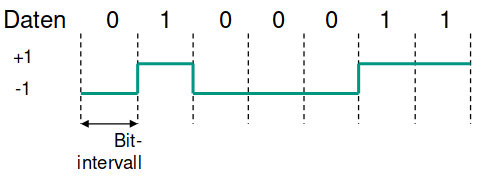
\includegraphics[width=0.6\textwidth]{images/03-nrz.png}
		\end{center}
		\caption{NRZ-Codierung des Wortes 010001}
	\end{figure}

	Die Baudrate ist bei NRZ recht niedrig (Signalwertwechsel nur bei 0-1- bzw. 1-0-Übergängen).
	Taktrückgewinnung ist bei längeren 0- oder 1-Folgen jedoch nicht möglich.

	\subsubsection{Manchester}

	Der Manchester-Code ist ein sogenannter Biphasen-Code: Symbolwerte werden durch Phasensprünge bestimmt.
	Eine 1 (0) in der Nachricht wird als Signalübergang vom hohen Pegel zum niedrigen Pegel (vom niedrigen zum hohen Pegel) in der Intervallmitte codiert.
	Bei 0-Folgen oder 1-Folgen müssen also \enquote{Hilfswechsel} eingefügt werden, um mehrfache Phasensprünge in derselben Richtung zu ermöglichen.

	\begin{figure}
		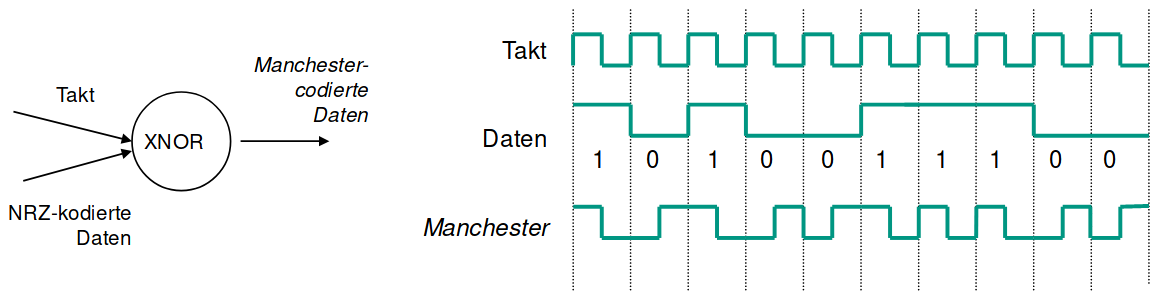
\includegraphics[width=\textwidth]{images/03-manchester.png}
		\caption{Manchester-Codierung des Wortes 1010011100}
	\end{figure}

	Taktrückgewinnung lässt sich beim Manchester-Code recht einfach umsetzen, da mindestens ein Signalwertwechsel pro Taktintervall auftritt.
	Die Baudrate ist jedoch sehr hoch; bei 0-Folgen oder 1-Folgen ist sie doppelt so hoch wie die Datenrate.
	Die Implementierung des Manchester-Codes ist einfach; er ist die XNOR-Verknüpfung der Daten und des Taktes.

	\subsubsection{AMI}

	AMI (Alternate Mark Inversion) nutzt einen ternären Code mit den möglichen Werten -1, 0 und 1.
	Eine 0 in der Nachricht wird als 0 über ein gesamtes Taktintervall codiert.
	Eine 1 wird abwechselnd als -1 und 1 über ein gesamtes Taktintervall codiert.

	\begin{figure}
		\begin{center}
			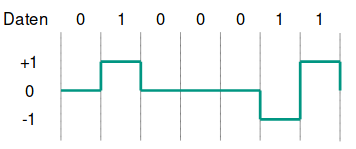
\includegraphics[width=0.6\textwidth]{images/03-ami.png}
		\end{center}
		\caption{AMI-Codierung des Wortes 0100011}
	\end{figure}

	Taktrückgewinnung ist bei AMI bei langen 0-Folgen nicht möglich.
	Die Baudrate ist bei AMI einigermaßen niedrig (Signalwertwechsel an 0-1, 1-0 und 1-1-Übergängen aber nicht bei 0-0).

	\subsection{Störquellen}

	Wie bereits erwähnt kann eine Störquelle das Signal auf einem Kanal beeinflussen.
	Wichtige Beeinträchtigungen sind:

	\begin{itemize}
		\item \emph{Dämpfung} (Attenuation)
		\item \emph{Verzögerung} (Delay Distortion)
		\item \emph{Rauschen} (Noise)
	\end{itemize}

	\subsubsection{Dämpfung}

	Die Stärke eines Signales sinkt mit zunehmender Distanz.
	Beschrieben in dB/m.
	Beim Empfänger muss die Signalstärke noch groß genug sein, um das Signal überhaupt zu erkennen und größer als das Rauschen.
	Dafür können Verstärker oder Repeater eingsetzt werden.

	\subsubsection{Verzerrung}

	Durch die Verzögerung der Signalausbreitung entsteht Verzögerungsverzerrung.
	Diese variiert mit der Frequenz.
	Da unterschiedliche Frequenzen den Empfänger zu verschiedenen Zeiten erreichen können, kann es zu Phasenverschiebung zwischen den Frequenzen.
	Aufeinanderfolgende Bits können dadurch überlappen.
	Dies nennt man \emph{Intersymbol-Interferenz}.

	\begin{figure}
		\begin{center}
			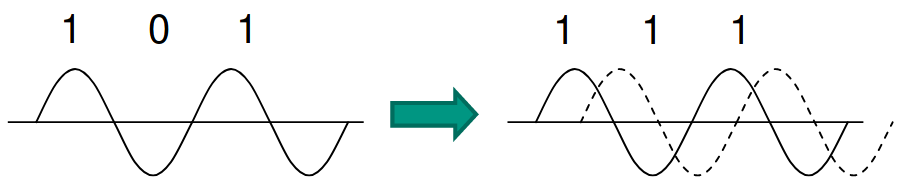
\includegraphics[width=0.6\textwidth]{images/03-intersymbol-interference.png}
		\end{center}
		\caption{Verzögerungsverzerrung (Intersymbol-Interferenz)}
	\end{figure}

	\subsubsection{Rauschen}

	\paragraph{Thermisches Rauschen}

	Thermisches Rauschen ist eine Funktion der Temperatur.
	Es ist gleich verteilt über Frequenzen hinweg (\enquote{weißes Rauschen}) und kann nicht eliminiert werden.
	Es bestimmt damit die maximales Leistungsfähigkeit.

	\paragraph{Modulationsrauschen}

	Zwei Frequenzen überlagern sich.

	\paragraph{Impulsrauschen}

	Impulsrauschen wird hervorgerufen von elektromagnetischen Störungen wie bspw. Blitzen.
	Es macht sich bemerkbar durch unregelmäßige Ausschläge und Geräuschspitzen kurzer Dauer und hoher Amplitude.

	\begin{figure}
		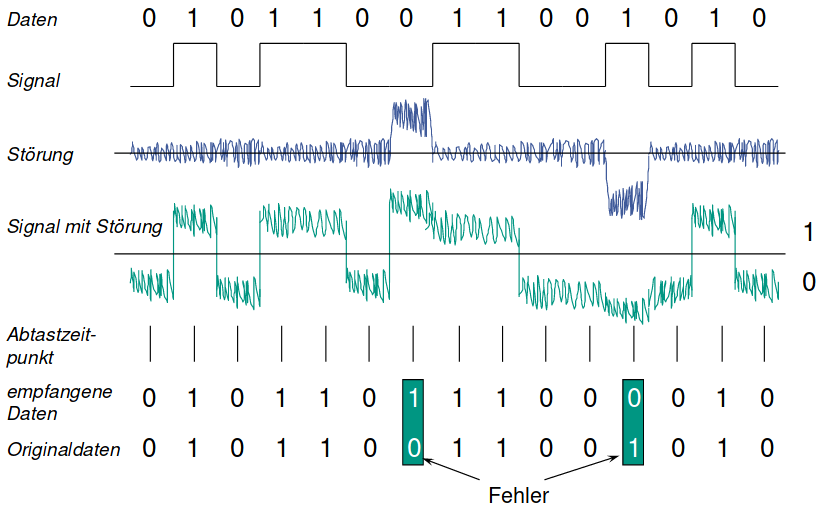
\includegraphics[width=\textwidth]{images/03-error.png}
		\caption{Auswirkung von Störungen}
	\end{figure}

	\section{Sicherungsschicht}

	Die Sicherungsschicht basiert auf den Diensten der physischen Schicht.
	Diese stellen unzuverlässige Übertragung von Bitfolgen bereit; es ist also nicht garantiert, dass Bits fehlerfrei übertragen werden.

	Die Sicherungsschicht bietet:

	\begin{itemize}
		\item Dienste zur zuverlässigen und unzuverlässigen Übertragung; zur Bereitstellung zuverlässiger Dienste sind Erkennung und Behebung von Fehlern der physischen Schicht erforderlich.
		\item Adressierung benachbarter Geräte; an einem physischen Medium können mehrere Geräte angeschlossen sein (bspw. Bus).
		\item Pufferung von Daten sowohl im sendenden als auch im empfangenden Gerät.
		\item Abstraktion vom physischen Medium.
	\end{itemize}

	\subsection{Grundlegendes Szenario}

	\subsubsection{Broadcast- vs. Punkt-zu-Punkt-Link}

	\paragraph{Broadcast-Link}

	Alle an ein Broadcast-Medium angeschlossenen Geräte empfangen auf diesem Medium übertragene Rahmen.

	\paragraph{Punkt-zu-Punkt-Link}

	Zwei Geräte sind über einen dedizierten Link verbunden.

	\subsubsection{Punkt-zu-Punkt-Link}

	An einem Punkt-zu-Punkt-Link sind die Kommunikationsformen Simplex, Duplex und Halbduplex möglich.

	\paragraph{Simplex}

	Übertragung nur in eine Richtung.

	\paragraph{Duplex}

	Zeitgleiche Übertragung in beide Richtungen (auch \emph{Vollduplex}).

	\paragraph{Halbduplex}

	Abwechselnde Übertragung in beide Richtungen.

	\subsubsection{Annahmen}

	In diesem Kapitel gehen wir von folgendem Szenario aus:
	Zwei Geräte $A$ und $B$ sind direkt über ein physisches Medium miteinander verbunden.
	Das verwendete Medium ist ein Vollduplex-Punkt-zu-Punkt-Link.

	\subsection{Bitfehler}

	Während der Übertragung einer Bitfolge kann es zur Verfälschung von Bits kommen.
	Fehlerursachung können beispielsweise Störungen auf der physischen Schicht sein.

	\paragraph{Einzelbitfehler}

	Ein einzelnes Bit ist fehlerhaft.

	\paragraph{Bündelfehler}

	Mehrere direkt aufeinanderfolgende Bits sind fehlerhaft.

	\subsubsection{Bitfehlerrate}

	Die Bitfehlerrate ist ein Maß für die Fehlerhäufigkeit.
	Sie wird durch das Verhältnis gestörter Bits zu übertragenen Bits berechnet:

	\begin{equation*}
		\text{Bitfehlerrate} = \frac{\sum \text{gestörte Bits}}{\sum \text{übertragene Bits}}
	\end{equation*}

	Typische Werte für die Bitfehlerrate sind:

	\begin{itemize}
		\item Analoges Fernsprechnetz: $2 \times 10^{-4}$ $\approx$ $0,02\%$
		\item Funkstrecke: $10^{-3}$ bis $10^{-4}$ $\approx$ $0,1\%$ bis $0,01\%$
		\item Ethernet: $10^{-9}$ bis $10^{-10}$ $\approx$ $0,0000001\%$ bis $0,00000001\%$
		\item Glasfaser: $10^{-10}$ bis $10^{-12}$ $\approx$ $0,00000001\%$ bis $0,0000000001\%$
	\end{itemize}

	% TODO: Fehlerauswirkungen (?)

	\subsection{Paketfehler}

	Es gibt vier Arten von Paketfehlern:

	\paragraph{Verlust eines Pakets}

	Das Paket wird erfolgreich versendet, kommt aber nicht beim Empfänger an.
	Grund dafür können Störungen des Mediums sein.

	\paragraph{Duplizierung eines eines Pakets}

	Das Paket wird einmal versendet, kommt aber mehrmals beim Empfänger an.
	Grund dafür können Störungen des Mediums sein.

	\paragraph{Empfang eines Phantom-Pakets}

	Das Paket kommt beim Empfänger an, wurde aber nicht vom (korrekten) Sender versendet.
	Gründe dafür können verfrühte Sendewiederholung des Senders oder falsche Zustellung sein.

	\paragraph{Reihenfolgevertauschung}

	Zwei oder mehr Pakete kommen in einer anderen Reihenfolge beim Empfänger an, als in der, in der sie versendet worden sind.
	Ein Grund dafür kann sein, dass die Pakete verschiedene Wege durch das Weg nehmen.

	\subsection{Kanalcodierung}

	Im \hyperref[sec:shannon]{abstrakten Modell nach Shannon} sitzt der \emph{Kanalcodierer} zwischen Informationsquelle und Sender.
	Er schützt Daten durch Hinzufügen von Redundanz gegen Übertragungsfehler.

	\subsubsection{Redundanz}

	Redundanz wird in Rechnernetzen auf verschiedene Weisen genutzt.

	\paragraph{Fehlererkennung}

	Durch Hinzufügen von Redundanz wird der Unterschied zwischen Codewörtern erhöht.
	Ein Beispiel aus der Realität ist das NATO-Alphabet.
	Da bspw. T und D über Funk schwer zu unterscheiden sind, sagt man \enquote{Tango} und \enquote{Delta}.
	Einen Fehlererkennungscode nennt man auch \emph{Error Detecting Code} (EDC).

	\paragraph{Fehlerkorrektur}

	Werden Fehler erkannt, können mittels der hinzugefügten Redundanz korrigiert werden.
	Dies nennt man auch \emph{Forward Error Correction} (FEC).

	\paragraph{Wiederholungsaufforderung}

	Der Empfänger teilt dem Sender das Ergebnis der Fehlerkorrektur mit.
	Der Sender wiederholt gegebenenfalls die Übertragung der Daten.
	Dies nennt man \emph{Automatic Repeat Request} (ARQ).

	\subsubsection{Fehlererkennender, -korrigierender Code}

	\paragraph{Fehlererkennender Code}

	Ein Code ist $r$-fehlererkennend, wenn der Empfänger jedes Codewort, in dem bis zu $r$ Symbole verfälscht wurden, als fehlerhaft identifizieren kann.

	\paragraph{Fehlerkorrigierender Code}

	Ein Code ist $r$-fehlerkorrigierend, wenn der Empfänger jedes Codewort, in dem bis zu $r$ Symbole verfälscht wurden, wiederherstellen kann.

	% TODO: Hamming-Abstand, Code-Abstand, Hamming-Kugel

	\subsection{Erkennung von Bitfehlern}

	Im folgenden gelte:

	\begin{align*}
		\text{Nutzdaten: } x &= x_1 \cdot x_2 \cdot ... \cdot x_k
	\end{align*}

	\subsubsection{Einfache Paritätsprüfung}

	\begin{align*}
		\text{Paritätsbit: } p &= x_1 \oplus x_2 \oplus ... \oplus x_k \\
		\text{Codewort: } z &= x \cdot p
	\end{align*}

	Beispielsweise wird das Wort $x = 1010$ codiert als $z = 10100$.
	Der Empfänger erhält $z* = 11100$ mit einem Bitfehler an der zweiten Stelle.
	Er erkennt den Fehler, da das Paritätsbit von $z*$ $p* = 1$ nicht mit dem ursprünglichen Paritätsbit $p = 0$ übereinstimmt.

	Einfache Paritätsprüfung erkennt nur einzelne Bitfehler.

	\subsubsection{Hamming-Code}

	An denjenigen Stellen, die Zweierpotenzen sind, stehen im Codewort Paritätsbits.
	Die restlichen Stellen werden mit den Nutzdaten aufgefüllt.

	\begin{align*}
		\text{Nutzdaten: } x &= 1000, k = 4 \\
		\text{Codewort: } z &= p_1 \cdot p_2 \cdot x_1 \cdot p_3 \cdot x_2 \cdot x_3 \cdot x_4 = p_1 \cdot p_2 \cdot 1 \cdot p_3 \cdot 0 \cdot 0 \cdot 0 \\
		\text{Paritätsbits: } p_k &= \bigoplus_{e \in E_k} e, E_k = \{ z_i : i \neq 2^{k-1} \wedge i = 2^{k-1} + j \times 2^{k} + l, j \in \mathbb{N}_0, l \in [0; 2^k) \subseteq \mathbb{N}_0 \} \\
		p_1 &= z_3 \oplus z_5 \oplus z_7 = x_1 \oplus x_2 \oplus x_4 = 1 \\
		p_2 &= z_3 \oplus z_6 \oplus z_7 = x_1 \oplus x_3 \oplus x_4 = 1 \\
		p_3 &= z_5 \oplus z_7 \oplus z_8 = x_2 \oplus x_3 \oplus x_4 = 0 \\
		\Rightarrow z &= 1110000
	\end{align*}

	Das Paritätsbit $p_k$ berechnet sich aus der XOR-Verknüpfung einiger Stellen des Codeworts.
	Dazu gehören die $2^{k-1} - 1$ nachfolgenden Stellen; dann werden $2^{k-1}$ Stellen übersprungen, die nächsten $2^{k-1}$ Stellen gezählt, $2^{k-1}$ Stellen übersprungen etc.
	Im obigen Beispiel folgen auf $p_1$ bspw. $2^0 - 1 = 0$ Bits, dann wird eine ($2^{k-1} = 1$) Stelle übersprungen ($z_2$), eine Stelle gezählt ($z_3$), eine Stelle übersprungen ($z_4$) und auf gleiche Weise werden noch die Stellen $z_5$ und $z_7$ gezählt.
	Diese Stellen des Codeworts entsprechen den Stellen $x_1$, $x_2$ und $x_4$ der Nutzdaten.
	Das Paritätsbit $p_1$ ist also $1 \oplus 0 \oplus 0 = 1$.

	\paragraph{Korrektur von Bitfehlern}
	
	Der Hamming-Code kann Bitfehler korrigieren.
	Um die Position eines Bitfehlers zu finden, berechnet der Empfänger aus $z^*$ (dem womöglich verfälschten Codewort) die Paritätsbits von $x^*$.
	Die XOR-Verknüpfung dieser berechneten Paritätsbits $q^*$ mit den empfangenen Paritätsbits $p^*$ liefert die Position des Bitfehlers.

	Sei beispielsweise das gesendete Codewort $z = 1110000$ und das empfangene Codewort $z^* = 1110010$.
	Es ist also ein Bitfehler an der 6. Position aufgetreten.
	Dann gilt:

	\begin{align*}
		z^* &= z^*_1 \cdot ... \cdot z^*_7 = p^*_1 \cdot p^*_2 \cdot x^*_1 \cdot p^*_3 \cdot x^*_2 \cdot x^*_3 \cdot x^*_4 \\
		x^* &= x^*_1 \cdot ... \cdot x^*_4 = 1010 \\
		q^*_1 &= x^*_1 \oplus x^*_2 \oplus x^*_4 = 1 \\
		q^*_2 &= x^*_1 \oplus x^*_3 \oplus x^*_4 = 0 \\
		q^*_3 &= x^*_2 \oplus x^*_3 \oplus x^*_4 = 1 \\
		\Rightarrow q^* &= q^*_3 \cdot q^*_2 \cdot q^*_1 = 101 \\
		p^* &= p^*_3 \cdot p^*_2 \cdot p^*_1 = 011 \\
		q^* \oplus p^* &= 110_2 = 6_{10}
	\end{align*}

	Ist die XOR-Verknüpfung von $q^*$ und $p^*$ Null, wurde das Codewort fehlerfrei übertragen.

	\subsubsection{Cyclic Redundancy Check}

	% TODO

	\subsection{Vorwärtsfehlerkorrektur}

	Vorwärtsfehlerkorrektur (FEC) setzt neben fehlerkorrigierenden Codes zusätzlich redundante Pakete/Rahmen ein, um es dem Empfänger zu ermöglichen, Paketfehler zu korrigieren ohne Sendewiederholungen anfordern zu müssen.
	Dies reduziert im Allgemeinen die Verzögerung bis Daten beim Dienstnutzer abgeliefert werden können.
	Andererseits werden die redundanten Pakete unabhängig davon gesendet, ob ein tatsächlich ein Fehler auftritt.
	Dadurch sinkt die für Nutzdaten einsetzbare Bandbreite.

	Seien beispielsweise die Pakete $D_1 = 0101$, $D_2 = 1111$ und $D_3 = 0000$ zu senden.
	Durch den Einsatz fehlererkennender Codes ist es dem Empfänger möglich, zu entscheiden, ob ein erhaltenes Paket fehlerbehaftet ist.
	Über die XOR-Verknüpfung berechnet der Sender nun ein zusätzliches Paket $K = D_1 \oplus D_2 \oplus D_3 = 1010$.
	Der Empfänger muss nur drei dieser vier Pakete korrekt empfangen.

	Wird bspw. Paket $D_1$ nicht empfangen, kann der Empfänger dieses aus der XOR-Verknüpfung der restlichen (korrekt empfangenen) Pakete $D_1 = K \oplus D_2 \oplus D_3$ rekonstruieren; dasselbe gilt für $D_2$ und $D_3$.
	Fehlt $K$, so sind die restlichen Pakete korrekt übertragen worden.

	Fehlt mehr als ein Paket, so muss eine Sendewiederholung beantragt werden.

	\subsection{ARQ-Verfahren}

	Unter ARQ (Automatic Repeat Request) werden Verfahren zur Sendewiederholung bei Paketfehlern zusammengefasst.
	Verfahren unterscheiden sich beispielsweise in der Art der verwendeten Quittungen, wann Quittungen versendet und Sendewiederholungen veranlasst werden oder wieviele Daten der Sender versenden darf, ohne eine Quittung erhalten zu haben.

	\subsubsection{Leistungsbewertung}

	Zur Bewertung von ARQ- und im allgemeinen Übertragungsverfahren gibt es verschiedene Kriterien.

	\paragraph{Durchsatz/Datenrate}

	Die Datenrate (\emph{Throughput}) $r$ ist ein Maß für die Menge an Daten, die pro Zeiteinheit übertragen werden können.
	Sie wird in bit/s angegeben.

	\paragraph{Sendezeit}

	Die Sendezeit (\emph{Transmission Delay}) ist die Zeit, die nötig ist um $n$ Bits zu senden.
	Sie ist abhängig von der Datenrate.

	\paragraph{Ausbreitungsverzögerung}

	Die Ausbreitungsverzögerung (\emph{Propagation Delay}) $t_a$ ist die Zeit, die ein Bit von A nach B benötigt.
	Anders gesagt erfasst sie die Zeitspanne zwischen Absenden eines Signals und dessen Eintreffen am anderen Ende des Mediums.
	Sie ist abhängig von der \enquote{Länge} des Medium un der Ausbreitungsgeschwindigkeit.

	\begin{equation*}
		t_a = \frac{d}{v}
	\end{equation*}

	Hier bezeichnet $d$ die Länge des Mediums in m, $v$ die Ausbreitungsgeschwindigkeit in m/s und $t_a$ die Ausbreitungsverzögerung in $s$.
	In üblichen Medien ist die Ausbreitungsgeschwindigkeit $v$ etwa zwei Drittel der Lichtgeschwindigkeit.

	Beispielsweise wäre für ein Medium der Länge $d = 500 \text{km}$ mit der Ausbreitungsgeschwindigkeit $v = 200000 \text{km/s}$ Ausbreitungsverzögerung $t_a = \frac{500 \text{km}}{200000 \text{km/s}} = 2,5 \text{ms}$.

	\paragraph{Sendezeit}

	Die Sendezeit $t_s$ ist die für den Sendevorgang beim Sender erforderliche Zeit.

	\begin{equation*}
		t_s = \frac{X}{r}
	\end{equation*}

	Hier bezeichnet $X$ die zu sendende Datenmenge in bit, $r$ die zur Verfügung stehende Datenrate in bit/s und $t_s$ die Sendezeit in $s$.

	\paragraph{Auslastung}

	Die Auslastung (\emph{Utilization}) $U$ ist ein Maß für die Nutzung einer Ressource (z.B. Übertragungsmedium).
	Sie beschreibt das Verhältnis der tatsächlichen Nutzung zur möglichen Nutzung der Ressource.

	\begin{equation*}
		U = \frac{t_s}{t_{Ges}}
	\end{equation*}

	\paragraph{Parameter $a$}

	Der Paramter $a$ ist definiert als:

	\begin{equation*}
		a = \frac{t_a}{t_s}
	\end{equation*}

	Er repräsentiert das Verhältnis der Länge des Mediums in Bit zur Länge eines Pakets.

	\paragraph{Bandbreiten-Verzögerungs-Produkt}

	\begin{itemize}
		\item Bandbreite $\times$ Verzögerung
		\item Bandbreite $\times$ RTT/2
	\end{itemize}

	\begin{equation*}
		\text{BVP} = t_a \times r = \frac{d}{v}r
	\end{equation*}

	Hier bezeichnet $d$ die Länge des Mediums in \si{\meter}, $v$ die Ausbreitungsgeschwindigkeit in \si{\meter\per\second} und $r$ die Datenrate in \si{\bit\per\second}.

	Seien beispielweise für eine WLAN-Verbindung die Datenrate/Bandbreite $r = \text{\SI{54}{\mega\bit\per\second}}$, die Entfernung $d = \text{\SI{50}{\meter}}$ und die Round-Trip-Time $\text{RTT} = \text{\SI{0,33}{\micro\second}}$.
	Das Bandbreiten-Verzögerungs-Produkt wäre dementsprechend:

	\begin{align*}
		\text{BVP} = t_a \times r = \frac{\text{RTT}}{2} \times r &= \frac{\text{\SI{0,33}{\micro\second}}}{2} \times \text{\SI{54}{\mega\bit\per\second}} \\
		&\approx \text{\SI{9}{\bit}}
	\end{align*}

	\paragraph{Weitere Kriterien}

	Die Kriterien Verarbeitungsverzögerung (\emph{Processing Delay}) $t_V$ und Warteschlagenverzögerung (\emph{Queuing Delay}) $t_Q$ sollen hier zwar genannt sein, werden im Folgenden aber vernachlässigt.

	\subsubsection{Stop-and-Wait}

	Stop-and-Wait ist ein sehr einfaches ARQ-Verfahren.
	Der Sender sendet ein Paket und wartet auf eine Quittung des Empfängers.
	Erst wenn die Quittung beim Sender angekommen ist, wird das nächste Paket gesendet.
	Empfängt der Sender nach einer bestimmten Wartezeit keine Quittung, sendet er das Paket erneut.
	Stop-and-Wait wird beispielsweise bei WLAN eingesetzt.

	Bei diesem Verfahren stellt sich üblicherweise die Frage, nach welcher Wartezeit eine Sendewiederholung erfolgen soll.

	\subsubsection{Alternating Bit Protocol}

	Durch irrtümliche Sendewiederholung (wenn bspw. die Quittung verloren geht) besteht die Möglichkeit, dass der Empfänger ein Paket doppelt erhält.
	Damit er diesen Fall erkennen kann, wird jedes Paket $P_i$ mit einer Sequenznummer $s(P_i)$ versehen, für die gilt:

	\begin{equation*}
		s(P_i) = s(P_{i-1}) + 1
	\end{equation*}

	Um das oben beschriebene Problem für Stop-and-Wait zu lösen, reicht eine Sequenznummer von einem Bit.
	Es muss nur unterschieden werden können, ob das erhaltene Paket ein gerades oder ungerades ist.
	Diese Stop-and-Wait-Variante nennt man Alternating Bit Protocol (ABP).

	\begin{figure}
		\begin{center}
			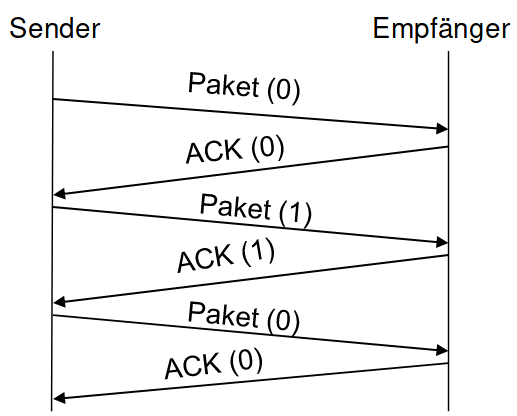
\includegraphics[width=0.6\textwidth]{images/04-stop-and-wait.png}
		\end{center}
		\caption{Stop-and-Wait mit 1-Bit-Sequenznummern (Alternating Bit Protocol)}
	\end{figure}

	Zusätzlich wird CRC zur Prüfung von Bitfehlern verwendet.
	Der Empfänger verwirft Pakete mit ungültiger CRC.

	\paragraph{Bewertung}

	Für ABP/Stop-and-Wait gilt für die Gesamtübertragungsdauer eines Pakets (unter Vernachlässigung der Verarbeitungszeiten, Sendezeit der Quittung, etc.):

	\begin{align*}
		t_{Ges} &= t_s(\text{Daten}) + t_a + t_V(\text{Daten}) + t_s(\text{Quittung}) + t_a + t_V(\text{Quittung}) \\
		&\approx t_s(\text{Daten}) + 2t_a
	\end{align*}

	Die Auslastung ist also:

	\begin{align*}
		U &= \frac{t_s}{t_{Ges}} = \frac{t_s}{t_s + 2t_a} = \frac{1}{1 + 2t_a/t_s} \\
		&= \frac{1}{1 + 2a}
	\end{align*}

	% TODO: weiter ausführen, siehe folien

	\subsubsection{Go-Back-N}

	Go-Back-N ist eine Generalisierung des Stop-and-Wait-Verfahrens zur Erhöhung der Leistungsfähigkeit.
	Der Sender kann hier mehrere Pakete versenden, bis er eine Quittung erhalten muss.
	Die maximale Anzahl nicht quittierter Pakete ist typischerweise durch das sogenannte Sendefenster $W$ begrenzt (für $W = 1$ ist Go-Back-N identisch mit Stop-and-Wait).
	Der Empfänger quittiert den Empfang eines Pakets i.d.R. mit einer kumulativen Quittung (\enquote{ich habe dieses Paket und alle vorhergehenden erhalten}).
	
	Wird ein Paket empfangen, das fehlerhaft oder außerhalb der Reihenfolge ist, wird es vom Empfänger verworfen.
	Der Sender hält für jedes gesendete Paket einen Timeout; läuft dieser für ein bestimmtes Paket ab, springt er in der Übertragungsreihenfolge zu diesem Paket zurück.

	Dies bedeutet, dass mindestens der Sender einen Paketpuffer für diejenigen Pakete bereitstellen muss, deren Sendung eventuell wiederholt werden muss.
	Auch der Empfänger kann mit einem Puffer arbeiten, wenn Pakete nicht direkt an die darüberliegende Schicht weitergeleitet werden können.

	\paragraph{Bewertung}

	Man unterscheidet bei der Bewertung des Go-Back-N-Verfahrens:

	\begin{itemize}
		\item Fenstergröße $W \geq 1 + 2a$: Der Sender kann ohne Pause senden; der Übertragungsabschnitt ist zu 100 \% ausgelastet.
		\item Fenstergrüße $W < 1 + 2a$: Sender kann nach dem \enquote{Aufbrauchen} des Fenster nicht weiter senden.
	\end{itemize}

	Für die erzielbare Auslastung gilt also:

	\begin{equation*}
		U = \begin{cases}
			1 & \text{für } W \geq 1 + 2a \\
			\frac{W}{1 + 2a} & \text{sonst}
		\end{cases}
	\end{equation*}

	\subsubsection{Selective Repeat}

	Anders als bei Go-Back-N werden vom Empfänger selektive (nicht kumulative) Quittungen erteilt.
	Pakete, die außerhalb der Reihenfolge empfangen werden, puffert der Empfänger, bis alle vorhergehenden Pakete empfangen wurden.
	Läuft der Timeout für die Quittung eines Pakets beim Sender ab, wird diese erneut gesendet.

	Selective Repeat reduziert das Datenaufkommen im Vergleich zu Go-Back-N, da im Fehlerfall nur einzelne Pakete wiederholt werden.

	\subsubsection{Selective Reject}

	Selective Reject verhält sich bis auf das Quittierungsverhalten des Empfängers identisch zu Selective Repeat.
	Statt eines Timeouts auf der Seite des Senders wird jedoch der Empfänger selbst aktiv, wenn er merkt, dass ein Paket fehlt.
	Empfängt er ein Paket, dessen vorhergehende Pakete nicht (korrekt) empfangen wurden, sendet er eine spezielle \enquote{negative} Quittung (SREJ(Sequenznummer)) für jedes fehlende Paket.
	Empfängt der Sender eine solche negative Quittung, wiederholt er sofort das Paket, statt auf einen Timeout zu warten.

	\subsection{Flusskontrolle}

	Ein Problem, das (nicht nur) auf der Sicherungsschicht auftreten kann, ist, das der Empfänger vom Sender überlastet werden kann.
	In diesem Fall müssen Pakete verworfen werden, da der Empfangspuffer nicht ausreichend groß ist.
	Der Sender sollte also die Größe des Empfangspuffers berücksichtigen.

	\paragraph{Closed-Loop-Flusskontrolle}

	Rückkopplung, um zu verhindern, dass der Empfänger überschwemmt wird.
	Der Sender adaptiert seinen Datenstrom entsprechend.

	Diese Variante der Flusskontrolle wird im Folgenden betrachtet.
	Sie wird im Internet eingesetzt.

	\paragraph{Open-Loop-Flusskontrolle}

	Beschreibung des Verkehrs in Richtung des Empfängers, anschließende Ressourcenreservierung und Überwachung des eingehenden Verkehrs.

	Diese Variante wird im Internet i.d.R. nicht eingesetzt und soll hier nicht weiter betrachtet werden.

	\subsubsection{Halt-und-Weiter}

	Bei Halt-und-Weiter kann der Empänger dem Sender die Meldungen \enquote{Halt} und \enquote{Weiter} senden.
	\enquote{Halt} bedeutet dem Sender, dass der Empfänger nicht mehr schritthalten kann; \enquote{Weiter} bedeutet ihm nach einer \enquote{Halt}-Meldung, dass der Empfänger wieder bereit ist.
	
	Halt-und-Weiter wird beispielsweise bei Fast-Ethernet oder Gigabit-Ethernet eingesetzt.

	\paragraph{Bewertung}

	\begin{itemize}
		\item Nur auf Vollduplex-Links einsetzbar.
		\item Bei hoher (Ausbreitungs-)Verzögerung nicht effektiv.
		\item Probleme bei Verlust der \enquote{Halt}-Meldung.
	\end{itemize}

	\subsubsection{Kreditbasierte Flusskontrolle}

	Der Sender kann nur eine begrenzte Menge Daten (Pakete/Bytes) senden, ohne eine Quittung erhalten zu haben.
	Diese Menge repräsentiert die Pufferkapazität des Empfängers.
	Sie wird \emph{Sendekredit} genannt.

	% TODO: sliding window if important

	\subsection{Verbindungen}

	Unter einer (Kommunikations-)Verbindung versteht man eine Kommunikationsbeziehung zwischen zwei oder mehreren Kommunikationspartnern.
	Eine Verbindung ist durch den bei den Kommunikationspartnern jeweils etablierten gemeinsamen (Verbindungs-)Kontext (bspw. Sequenznummern, Fenstergrößen) charakterisiert.

	Eine Verbindung stellt die Basis für die Bereitstellung zuverlässiger Dienste bereit.

	\paragraph{Verbindungsorientierte Kommunikation}

	\begin{itemize}
		\item Verbindungsaufbau (Etablierung eines Verbindungskontexts)
		\item Datenaustausch
		\item Verbindungsabbau (Löschen des Kontexts, Freigeben von Puffern, etc.)
	\end{itemize}

	Verbindungsorientierte Kommunikation hat den Vorteil, dass beim Aufbau der Verbindung die Parameter des Kontexts ausgehandelt werden können.
	Außerdem kann nur auf diese Weise ein zuverlässiger Dienst bereitgestellt werden.

	Der Aufbau der Verbindung verzögert jedoch auch den tatsächlichen Datenaustausch.
	Dies merkt man beispielsweise beim Abruf von Webseiten.
	Modernere Protokolle sehen Datenaustausch bereits während des Verbindungsaufbaus vor, um dem entgegenzuwirken.

	\paragraph{Verbindungslose Kommunikation}

	Der Datenaustausch findet sofort statt.
	Es wird kein Kommunikationskontext zwischen den Partnern etabliert.

	Diese Art der Kommunikation ist zwar schnell, jedoch unzuverlässig; es besteht keine Möglichkeit der Kontrolle, ob Daten überhaupt angekommen sind (unzuverlässiger Dienst).

	\subsubsection{2-Wege-Handshake}

	Zum Verbindungsaufbau sendet der Sender einen Connect-Request an den Empfänger und wartet auf dessen Bestätigung.

	\begin{figure}
		\begin{center}
			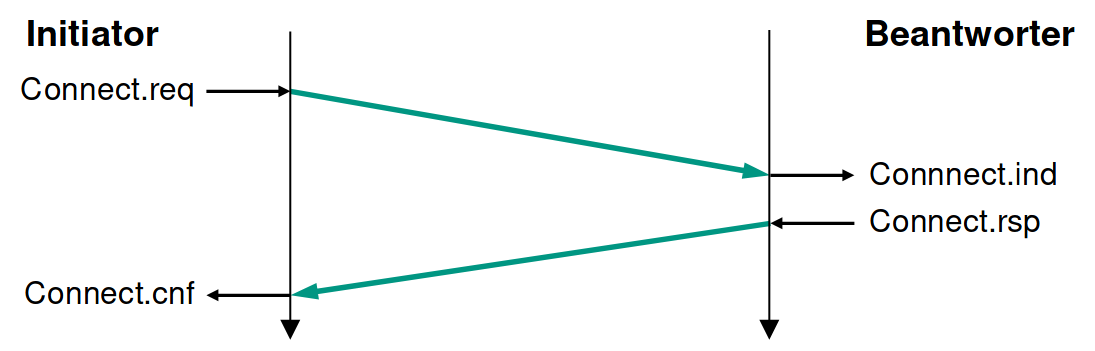
\includegraphics[width=0.6\textwidth]{images/04-2-way-handshake.png}
		\end{center}
		\caption{2-Wege-Handshake}
	\end{figure}

	Ein Problem an dieser Art des Verbindungsaufbaus besteht darin, dass der Empfänger bei Verlust dieser Bestätigung die Verbindung als hergestellt betrachtet, auch wenn sie es nicht ist.

	\subsubsection{3-Wege-Handshake}

	Dieses Problem löst der 3-Wege-Handshake durch eine erneute Bestätigung der Bestätigung seitens des Senders.

	\begin{figure}
		\begin{center}
			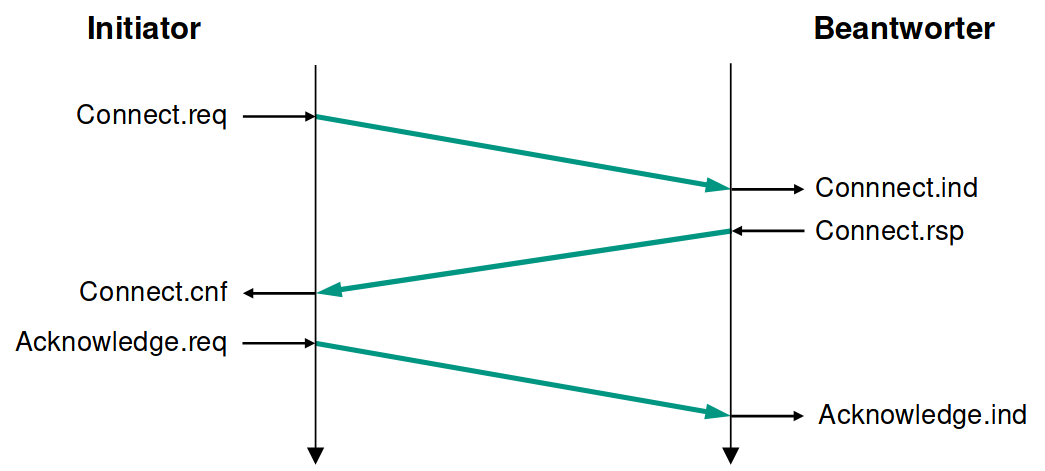
\includegraphics[width=0.6\textwidth]{images/04-3-way-handshake.png}
		\end{center}
		\caption{3-Wege-Handshake}
	\end{figure}

	\subsection{Netztopologien}

	\subsubsection{Vollvermaschtes Netz}

	In einem vollvermaschten Netz ist jedes Gerät physisch mit jedem anderen verbunden.
	Bei $n$ Geräten erfordert dies $\frac{n(n - 1)}{2} \in O(n^2)$ Links.
	Dieser Ansatz daher ist bei großen Netzen nicht einsetzbar.

	\subsubsection{Teilvermaschtes Netz}

	Im Gegensatz dazu sind in einem teilvermaschten Netz nur ein Teil der Geräte physisch verbunden.
	Kommunikation zwischen nicht verbundenen Geräten muss über Zwischensysteme erfolgen.

	\paragraph{Baum}

	Netzgraph ist in Baumform; Blätter sind Endsysteme bzw. Netzrand.
	Dieser Topologie wird bspw. im klassischen Telefonnetz eingesetzt.

	\begin{figure}
		\begin{center}
			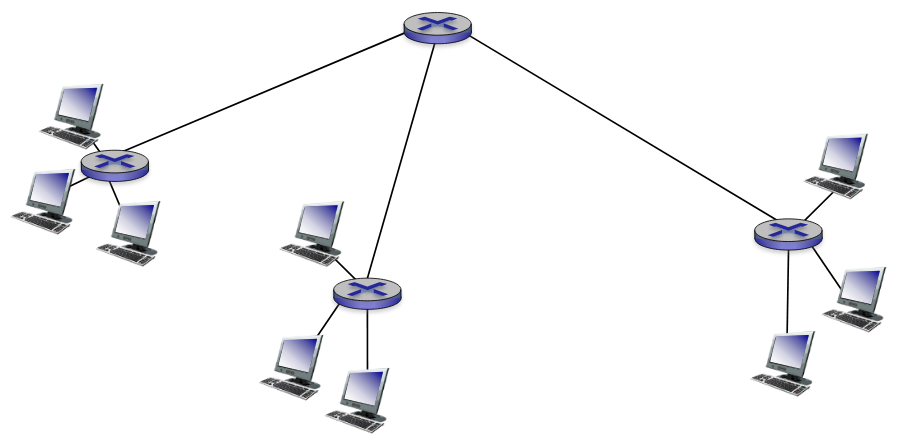
\includegraphics[width=0.6\textwidth]{images/04-tree-topology.png}
		\end{center}
		\caption{Baumtopologie}
	\end{figure}

	\paragraph{Stern}

	Baumtopologie, bestehend nur aus der Wurzel und den Blättern.
	Es gibt also genau eine zentrale Komponente, zu der jedes Gerät eine physische Verbindung hat.
	Diese Komponente ist ein sogenannter \enquote{single point of failure}.

	\paragraph{Ring}

	Der Netzgraph bildet einen einzigen Zyklus.
	Jedes Gerät ist also mit genau zwei anderen physisch verbunden.

	\begin{figure}
		\begin{center}
			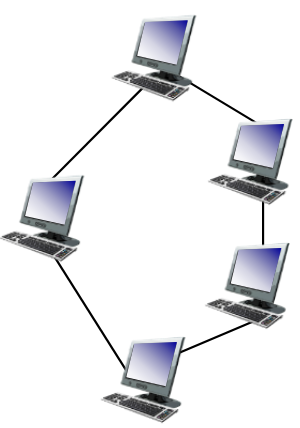
\includegraphics[width=0.3\textwidth]{images/04-ring-topology.png}
		\end{center}
		\caption{Ringtopologie}
	\end{figure}

	\paragraph{Bus}

	Alle Geräte sind über einen physischen Link verbunden (wie bspw. bei der MiMa).

	\begin{figure}
		\begin{center}
			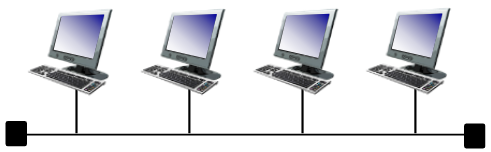
\includegraphics[width=0.3\textwidth]{images/04-bus-topology.png}
		\end{center}
		\caption{Bustopologie}
	\end{figure}

	\subsection{Multiplexverfahren}

	Unter Multiplexen versteht man die simultane Nutzung eines physischen Links durch mehrere Signale.
	Ziel dabei ist die optimale Nutzung der verfügbaren Ressourcen.

	\subsubsection{Raummultiplex}

	% TODO

	\subsubsection{Frequenzmultiplex}

	% TODO

	\subsubsection{Zeitmultiplex}

	Bei Zeitmulitplex (auch: Time Division Multiple Access, TDMA) wird die Zeit aufgeteilt in Abschnitte (Zeitschlitze, time slots), während deren die gesamte Bandbreite von einem Signal genutzt werden kann.
	Die Abschnitte können unterschiedlicher Länge sein und wiederholen sich i.d.R. periodisch.

	\paragraph{Statisch}

	Einteilung der Zeitschlitze erfolgt offline und ändert sich während des Betriebs nicht.
	Wird häufig in der Automatisierungstechnik (\enquote{Industrial Internet}) eingesetzt.

	\paragraph{Dynamisch-Fest}

	Während des Betriebs wird die Einteilung der Zeitschlitze über spezielle \enquote{Signalisierungsprotokolle} ausgemacht.
	Eingesetzt bspw. bei GSM (Sprach- und Datenübertragung).

	\paragraph{Dynamisch-Variabel}

	Zugriff erfolgt on-demand ohne Nutzung eines dedizierten Protokolls.
	Eingesetzt bspw. bei Ethernet oder WLAN.

	\subsubsection{Codemultiplex}

	% TODO

	\subsection{Medienzuteilung}

	\paragraph{Ausgangssituation}

	Häufiges Kommunikationsmuster: On-Off.
	On: Daten werden mit höchster verfügbarer Datenrate versendet.
	Off: es sind keine Daten zu senden.

	In der Regel ist die On-Zeit deutlich kürzer als die Off-Zeit.
	Außerdem ist es unklar, zu welchem Zeitpunkt eine On-Phase beginnt.
	Dies ist vergleichbar mit der Kommunikation über Telefon.

	In lokalen Netzen werden Verfahren zur variablen on-demand Medienzuteilung (Media Access Control, MAC) eingesetzt.

	\subsubsection{Aloha}

	% TODO

	Erstes MAC-Protokoll für paketbasierte drahtlose Netze.

	\begin{itemize}
		\item Zeitmultiplex, variabel, zufälliger Zugriff.
		\item Keine vorhergehende Medienüberprüfung/Ankündigung des Signals.
		\item Asynchroner Zugriff.
		\item Kollisionen möglich.
	\end{itemize}

	Aufgetretene Kolliosonen können auf verschiedene Weisen erkannt und behandelt werden:

	\begin{itemize}
		\item \emph{Explizite Kollisionserkennung} --- Höhere Schichten versenden Bestätigungen auf separatem Kommunikationskanal.
		\item \emph{Implizite Kollisionserkennung} --- Empfänger broadcastet empfangenes Signal an alle andere Geräte; Sender erhält in dieser Form eine Empfangsquittung.
	\end{itemize}

	Einer erkannten Kollision folgt i.d.R. eine Sendewiederholung.
	Da diese nicht wieder zu einer Kollision führen soll, wird ihr Zeitpunkt zufällig festgelegt.

	\paragraph{Slotted Aloha}

	Bei Slotted Aloha erfolgt zusätzlich eine Aufteilung in Zeitschlitze.
	Im Mittel hat Slotted Aloha weniger Kollisionen als Aloha.

	\subsubsection{CSMA}

	CSMA steht für Carrier Sense Multiple Access.
	Vor dem Senden eines Signals prüft der Sender, ob das Medium frei ist (\emph{Listen before Talk}, vgl. \enquote{Wenn ich rede hörst du zu}).
	Ist es belegt, versucht er es später wieder; ist das Medium frei, fängt er an zu senden.

	Auch hier kann es Kollisionen kommen, wenn zwei Sender gleichzeitig anfangen zu senden.

	\paragraph{CSMA-CD}

	Während des Sendens prüft der Sender, ob es auf dem Medium zu einer Kollision kommt (\emph{Listen while Talk}).
	Im diesem Fall wird das Senden abgebrochen und zu einem späteren Zeitpunkt erneut versucht.

	\paragraph{CSMA-CA}

	Sendende Station schließt bei Ausbleiben einer Quittung auf Kollision (bspw. WLAN).

	\subsubsection{Token Passing}

	% TODO

	\subsection{Ethernet}

	\subsubsection{Standardisierung}

	\subsubsection{Protokoll}

	\subsubsection{Kopplung von Ethernets}

	\subsubsection{Kollisionsdomäne}

	\subsubsection{Technische Varianten}

	\subsubsection{VLAN}

	\section{Vermittlungsschicht}

	\section{Transportschicht}

	\section{Anwendungsschicht}

	\section{Netzssicherheit}

	\section{Klausuraufgaben}
\end{document}
